\documentclass{sig-alternate}
\usepackage{url}
\usepackage{algorithm}
\usepackage[noend]{algorithmic}
\usepackage{subfigure}

\newcommand{\dae}{{\em Divide-and-Evolve}}
\newcommand{\DAE}{{\sc DaE}}
\newcommand{\DAEX}{{\sc DaE$_{\text{X}}$}}
\newcommand{\DAEYAHSP}{{\sc DaE$_{\text{YAHSP}}$}}
\newcommand{\YAHSP}{{\sc YAHSP}}
\newcommand{\PARADISEO}{{\sc ParadisEO}}
\newcommand{\OPENMP}{{\sc OpenMP}}
\newcommand{\OPENSTACKS}{{\sc Openstacks}}
\newcommand{\ELEVATORS}{{\sc Elevators}}

\pdfpagewidth=8.5in
\pdfpageheight=11in

\begin{document}

\conferenceinfo{GECCO'11,} {July 12--16, 2011, Dublin, Ireland.}
\CopyrightYear{2011}
\crdata{978-1-4503-0557-0/11/07}
\clubpenalty=10000
\widowpenalty = 10000

\title{Parallel Divide-and-Evolve:\\ Experiments with OpenMP on a Multicore Machine}

\numberofauthors{2} % 4 is a bug!

\author{
\alignauthor
Caner Candan\\
\affaddr{Thales Research \& Technology}\\
\affaddr{Palaiseau, France}\\
\email{caner.candan@thalesgroup.com}
\alignauthor
Johann Dr{\'e}o\\
\affaddr{Thales Research \& Technology}\\
\affaddr{Palaiseau, France}\\
\email{johann.dreo@thalesgroup.com}
\and
\alignauthor
Pierre Sav{\'e}ant\\
\affaddr{Thales Research \& Technology}\\
\affaddr{Palaiseau, France}\\
\email{pierre.saveant@thalesgroup.com}
\alignauthor
Vincent Vidal\\
\affaddr{ONERA -- DCSD}\\
\affaddr{Toulouse, France}\\
\email{vincent.vidal@onera.fr}
}

\maketitle
\begin{abstract}
Multicore machines are becoming a standard way to speed up the system performance.
After having instantiated the evolutionary metaheuristic \DAEX\ with the forward search \YAHSP\ planner, 
we investigate on the global parallelism approach, which exploits the intrinsic parallelism of the individual evaluation.
This paper describes a parallel shared-memory version of the \DAEYAHSP\ planning system using the \OPENMP\ directive-based API.
The parallelization scheme applies at a high level of abstraction and thus can be used by any evolutionary algorithm implemented with the Evolving Objects framework.
The proof of concept is validated on a 48-core machine with two planning tasks extracted from the last international planning competition.
Experiments show significant speedups with an increasing number of cores.
This preliminary work opens an avenue for parallelizing any evolutionary algorithm developed with EO that would target multicore architectures.
\end{abstract}

\category{I.2.8}{Artificial In\-tel\-ligen\-ce}{Problem Solving, Control Methods, and Search}%[Plan execution, formation, and generation]
\category{D.1.3}{Pro\-gramming Techniques}{Concurrent Programming}[Parallel Programming]
\terms{Algorithms, Experimentation, Performance.}
\keywords{Evolutionary Computation, Automated Planning, Parallel Shared-Memory, Multicore.\\\\} % NOT required for Proceedings

\section{Introduction}
The classical planning problem in Artificial Intelligence \cite{gnt04} is to find a path in a transition system: a sequence of actions which maps an initial
state $I$ into a state $G$ satisfying a set of desired goals. Usually, a metric is associated with the solution plan such as length, cost or duration (where
concurrent actions are allowed). In domain-independent planning, problems are described with the Planning Domain Description Language (PDDL) \cite{pddl:jair2003}. 
In the simplest STRIPS model, states of the world are defined by sets of atoms instantiated from a set of predicates and a set of
objects, and actions are triples of sets of atoms: preconditions, add effects, del effects. 
Instances of the planning problem, called planning tasks, can model many kinds of abstract reasoning problems and are known to be PSPACE-hard.

To solve such planning tasks, several heuristic search algorithms have been proposed in the past but none of them can be easily parallelized.
They require a great amount of work to provide efficiency while preserving correctness \cite{burns:JAIR2010,burns:ijcai2009}.

Recently, the \DAEX\ evolutionary metaheuristic has been proposed to solve such planning tasks \cite{dae:icaps2010,dae:evocop2006}.
As an evolutionary algorithm, \DAEX\ provides an intrinsic parallelism: the individual evaluation stage, which is often the most time-consuming stage during the evolutionary generation loop.
This nice property opens an avenue towards the design of a parallel planning system without going deeply inside a whole reconstruction of the sequential version.

Moreover, the implementation of \DAEX\ has been made with the STL-based Evolving
Objects framework\footnote{\url{http://eodev.sf.net}} which provides an abstract
control structure to develop any kind of evolutionary algorithm. Therefore, our
parallelization scheme is easily transposable to any evolutionary algorithm
developed within the EO framework.

As a proof of concept, we implemented a multi-threaded version of \DAEYAHSP, the
instantiation of \DAEX\ with the heuristic forward search \YAHSP\ planner
\cite{yahsp:icaps2004}, using the \OPENMP\ directive-based
API\footnote{\url{http://www.openmp.org}}. The design of experiment is built on
problems extracted from the last international planning
competition\footnote{\url{http://ipc.icaps-conference.org}} with the
multi-threaded \DAEYAHSP\ release mapped onto a 48-core parallel machine.

While clusters is the most common distributed memory system for high performance
computing, multicore architectures are gaining popularity as they become the
{\it de facto} standard in computer mass market. The GPGPU-based architectures
share similar characteristics, but require a specific programming language.
As a consequence we would have to rewrite entirely the \YAHSP\ solver called by our evaluation function.

The paper is outlined as follows. We first review related works in the
fields of parallel evolutionary computation and AI planning, before presenting
in more details the main algorithms on which our parallel system is based: the
evolutionary metaheuristic \DAEX\ and the forward-chaining heuristic search
planner YAHSP. The parallel implementation of \DAEYAHSP\ is then described, as
well as the specific problems, due to the shared-memory programming model, that
arose during this implementation. After having demonstrated the effectiveness
of our parallel implementation of \DAEYAHSP\ on two planning benchmark tasks, we
conclude and provide some insights of possible future works.

\section{Related Works}

\subsection{Parallel Evolutionary Algorithms}

A large literature deals with the parallelization techniques of Evolutionary
Algorithms (EAs). Depending on the targeted architecture, the parallelization
scheme may be chosen accordingly. The main approaches may be classified among:
simple {\it run level parallelism}, EA with {\it global parallelism} where the
evaluation stage is parallelized but not the other operators, and
{\it island-based} in which the population is partitioned into
separate subpopulations. These structured EAs further split into cellular
EAs (cEA) where the selection and reproduction steps are parallelized, and
distributed EAs {\it dEA} with a controlled migration between islands
\cite{alba:IEEE2002}.

The run level parallelism being trivially achieved by running several runs
concurrently, the first step when parallelizing a new algorithm is often to try
the global parallelization approach, because the evaluation step is often the
most costly part of EAs and because individual evaluations are generally
intrinsically independent.

A parallel extension of EO, \PARADISEO, has been proposed by Cahon et al.
\cite{paradiseo:JHeuristics2004}. It is based on the Message Passing Interface
(MPI) and proposes several parallelization schemes, available by calling
wrappers around common functions of EO. \PARADISEO\ targets multiprocessor
machines, especially clusters and grids, for running large-scale, general
purpose EAs. As we are targeting a multicore architecture, and since our
evaluation function has a large memory footprint, message passing may introduce
a time consuming memory copy overhead. This reason discards the \PARADISEO\
framework.

Another attractive parallel architecture is the GPGPU card with a very good
processor-price ratio. The work described in \cite{maitre:gecco2009} shows how a
simple general scheme can be designed for EAs, by parallelizing the evaluation
step. But the limitations that are pointed out can hardly be avoided in our
case. Firstly, without stack, functional calls are forbidden on a GPGPU card:
the whole code must be inlined; this would entail to inline the \YAHSP\
solver entirely, which would overcome the available length limit. Secondly,
it necessitates flat genome representations, which in our case would imply
a lot of copies of the atoms objects instances, which can be numerous on
large problems. Moreover, \YAHSP\ uses a memoization mechanism which is a
global shared-memory that save previous computations. It greatly speeds up
the search but cannot be used on a GPGPU because it may need up to several
gigabytes of memory on hard problems, where GPGPU cards have heavy
limitations on memory space. And finally speedups may be obtained for very large
sizes of population (e.g. 5000, 20000) which is not the average case here.
For these reasons we also discarded this type of architecture.

\subsection{Parallel Planning}
\label{section:previous-work}

Several approaches to parallel planning have been proposed in recent years.
Parallel Retracting A* \cite{PRA-star}, was implemented on a Connection Machine
and had to deal with very severe memory limitations. In that algorithm, a
distributed hash function is used to allocate generated states to a unique
processing unit and avoid unnecessary state duplications. PRA* deals with the
memory limitation through a retraction mechanism which allows a processor to free
its memory by dropping states. In order to confirm the transfer of a state,
synchronous communication channels must be used, which seriously slows down the
search process. Transposition-table driven work scheduling \cite{TDS}, similarly
to PRA*, uses a hash function to avoid duplication. It is based on IDA* and,
running on a standard architecture, does not necessitate any retraction
mechanism and can efficiently exploit asynchronous communication channels.
Parallel Frontier A* with Delayed Duplicate Detection \cite{PFADDD} uses a
strategy based on intervals computed by sampling to distribute the workload
among several workstations, targeting distributed-memory systems as opposed to
previous approaches. In \cite{HDA-star}, the authors introduce Hash Distributed
A* (HDA*) which combines successful ideas from previous parallel algorithms.
HDA* uses a hash function which assigns each generated state to a unique
processing unit in order to avoid the duplication of the search efforts. This
mechanism was introduced in PRA*, which unfortunately combined it with
synchronous communication channels which cause a lot of waiting. This problem
was addressed in HDA* by the use of non-blocking communication (as in
\cite{TDS}). In \cite{burns:ijcai2009,burns:JAIR2010} the authors present
Parallel Best-NBlock-First (PBNF). It uses an abstraction to partition the state
space. PBNF allows each thread to expand the most promising nodes while
detecting duplicate states. Rather than sleeping if a lock cannot be acquired, a
thread can perform ``speculative'' expansions by continuing the expansion of its
current part of the space. This technique keeps cores busy at the expense of
duplicate work. \cite{dovetailing} adapts for planning a technique called
dovetailing, in which several instances of a search algorithm with different
parameter settings are run in parallel. Finally, \cite{vidal:socs2010} proposed
a multicore version of the planner \cite{yahsp:icaps2004} where many concurrent
threads expand nodes from a common open list, yielding to early exploration of
branches of the search tree that would have been delayed by a classical search,
which can speedup search by several orders of magnitude.

\section{Methods}

\subsection{Algorithms}

\paragraph{Divide and Evolve}
\DAEX, the concrete implementation of the \dae\ paradigm, is a
domain-independent satisficing planning system based on Evolutionary Computation
\cite{dae:evocop2006}. The basic principle is to carry out a {\em
Divide-and-Conquer} strategy driven by an evolutionary algorithm. The algorithm
is detailed in \cite{dae:icaps2010} and compared with state-of-the-art planners.
In order to solve a planning task ${\cal P}_D(I,G)$, the basic idea of \DAEX\ is
to find a sequence of states $S_1, \ldots, S_n$, and to rely on an embedded
planner $X$ to solve the series of planning tasks ${\cal P}_D(S_{k},S_{k+1})$,
for $k \in [0,n]$ (with $S_0 = I$ and $S_{n+1} = G$). A \DAEX\ individual is a
sequence of goals which define a sequence of subproblems to be solved (a {\it
decomposition}). These subproblems are submitted successively to an embedded
planner $X$ and the global solution is obtained after the compression of these
intermediate solutions. The overall optimization process is controlled by
an evolutionary algorithm.

The fitness implements a gradient towards feasibility for unfeasible individuals
and a gradient towards optimality for feasible individuals. Feasible individuals
are always preferred to unfeasible ones. Population initialization as well as
variation operators are driven by the critical path $h^1$ heuristic
\cite{h1:aips2000} in order to discard inconsistent state orderings, and atom
mutual exclusivity inference in order to discard inconsistent states. Beside a
standard one-point crossover for variable length representations, four mutations
have been defined: addition (resp. removal) of a goal in a sequence, addition
(resp. removal) of an atom in a goal. The selection is a comparison-based
deterministic tournament of size 5.

For the sequential release, Darwinian-related parameters of \DAEX\ have been
fixed after some early experiments \cite{dae:evocop2006} whereas parameters
related to the variation operators have been tuned using the Racing method \cite{dae:gecco2010}.

All experiments were done with \DAEYAHSP: the instantiation of \DAEX\ with the \YAHSP\ heuristic forward search solver \cite{yahsp:icaps2004}. 
We added two novelties to the version described in \cite{dae:icaps2010}.
One important parameter is the maximum number of expanded nodes allowed to the \YAHSP\ sub-solver which defines empirically what is
considered as an easy problem for \YAHSP. As a matter of fact, the minimum number of required nodes varies from few nodes to thousands depending of the
planning task. In the current release this number is estimated during the population initialization stage. An incremental loop is performed until the
ratio of feasible individuals is over when a given threshold or a maximum boundary has been reached. By default this number is doubled at each iteration until at least
one feasible individual is produced or 100000 has been reached.

Furthermore we add the capability to perform restarts within a time contract in order to increase solution quality.

\paragraph{Yet Another Heuristic Search Planner}
The \YAHSP\ planning system \cite{yahsp:icaps2004} extends a technique introduced in the FF planner
\cite{ff:jair01} for calculating the heuristic, based on the extraction of
a solution from a planning graph computed for the relaxed problem obtained by
ignoring deletes of actions. It can be performed in polynomial time and space,
and the length in number of actions of the relaxed plan extracted from the
planning graph represents the heuristic value of the evaluated state. This
heuristic is used in a forward-chaining search algorithm to evaluate each
encountered state.

A novel way has been introduced in \YAHSP\ for extracting information from the
computation of the heuristic, by considering the high quality of the relaxed
plans extracted by the heuristic function in numerous domains. Indeed, the
beginning of these plans can often be extended to solution plans of the initial
problem, and there are often a lot of other actions from these plans that can
effectively be used in a solution plan. \YAHSP\ uses an algorithm for combining
some actions from each relaxed plan, in order to find the beginning of a valid
plan that can lead to a reachable state. Thanks to the quality of the extracted
relaxed plans, these states frequently guide search closer to a solution
state. The lookahead states thus calculated are then added to the list of nodes
that can be chosen to be expanded by increasing order of the numerical value of
the heuristic.

This lookahead strategy can be used in different search algorithms. In \YAHSP,
a classical best-first search algorithm has been modified in such a way that
completeness is preserved. It simply consists in augmenting the list of nodes
to be expanded (the open list) with some new nodes computed by the lookahead
algorithm. The branching factor is slightly increased, but the performances are
generally better and completeness is not affected.

A first motivation in the use of \YAHSP\ in \DAEX\ is that experiments about the
use of this lookahead strategy in a complete best-first search algorithm have
demonstrated that in numerous planning benchmark domains, the improvement of the
performance in terms of running time and size of problems that can be handled
are been drastically improved (cf. \cite{yahsp:icaps2004}). The \YAHSP\ planner
has been awarded a second place in the $4^{th}$ International Planning Competition
\cite{ipc4:jair05} and some recent results \cite{rintanen:acai2010} demonstrate
that it is still extremely competitive with more recent planners. A second
motivation in the use of \YAHSP\ in \DAEX\ is its ability to answer very fast to
the considerable number of planning requests emanating from \DAEX, as opposed to
modern techniques such as the landmark heuristics implemented in the LAMA
planner \cite{lama:jair2010} (winner of the $6^{th}$ International Planning
Competition) which require a costly analysis for each new initial state.

In order to speed up the search process, a memoization mechanism has been introduced in
\YAHSP\ and carefully controlled to leave memory space for \DAE. Indeed, most of
the time during a run of \YAHSP, and as a consequence during a run of \DAEYAHSP,
is spent in computing the $h^{add}$ heuristic for each encountered state. During a single run of YAHSP, duplicate states are discarded; but during a run of \DAEYAHSP, the same state can be encountered
multiple times. Therefore, we keep track of the $h^{add}$ costs of all atoms in
the problem for each state, in order to avoid recomputing these values each time
a duplicate state is reached. This generally leads to a speedup comprised
between 2 and 4. When \DAEYAHSP\ runs out of memory, which obviously happens
much faster with the memoization strategy, all stored states and associated
costs are flushed.
For the parallel scheme, we experimented two strategies: a global memoization shared by all individual evaluations against a memoization local to each individual evaluation. 
Results are presented in section \ref{section:results}.

\paragraph{Parts that can theoretically be parallelized}
As shown in section \ref{section:previous-work}, heuristic search algorithms
used in automated AI planners can be parallelized in many ways, although there
is no obvious and natural way to do so. However, our goal in this work is not
to parallelize the underlying planner, but the evolutionary algorithm which
controls the planner, which can be made in a very efficient way. Indeed, in
typical population-based algorithms such as evolutionary algorithms, the
evaluation of individuals can be made independently of each other, a fortiori in
a parallel way since there is no data-dependencies.
Applying variation operators can also be performed in parallel;
and depending on the application, parallelism on variation operators or
individual evaluation will have a different impact on the running time and
utilization of the computational resources.
In \DAEX, the running time of applying the variation operators is negligible w.r.t. the running time required
by the individual evaluations by an embedded planner, which is the reason why we only parallelized the latter.

\subsection{Implementation}

\paragraph{Locks, thread-Safe \& reentrant subroutines}
Even if being very natural in the context of evolutionary algorithms,
parallelizing individual evaluations in \DAEX\ requires to be carefully made in
order to avoid some typical problems that can happen with shared-memory parallel
implementations. Indeed, even if individual evaluations are made
independently of each other, some concurrent accesses to shared memory are still
required (for example, a basic one is incrementing some global counter),
especially in \YAHSP\ (detailed below). Furthermore, the original implementations of \DAEX\
and \YAHSP\ were not designed with parallelism in mind, which implied some
modifications to render them thread-safe.

One problem that can happen in a shared-memory parallel implementation is
\emph{deadlocks}, which are situations where at least two concurrent threads are
each waiting for the other one to finish, and thus neither ever does. This can
happen for example when a thread $t_1$ acquires a lock on a shared variable $x$,
and then tries to acquire a lock on another shared variable $y$; while in the
same time a thread $t_2$ acquired a lock on $y$ and then tries to acquire a lock
on $x$. Each thread waiting for the other one to release the lock on the next
variable locked by the other thread, nothing happens. A variation of deadlocks
is \emph{livelocks}, where the threads are still able to continue doing some
work but cannot go through some portion of the code due to a similar phenomenon.

Another problem that can arise is the concurrent use of a given subroutine by
several threads, when such a subroutine or some subroutines called, it modifies
some global data. This is a typical problem of reentrancy, which must be
carefully analyzed in order to render thread-safe a parallel implementation. Two
cases can then occur: either the global data must be shared by some threads, which
requires to protect its access, or it can be made private to each thread, thus
necessitating to change the scope of this data.

\paragraph{EO \& OpenMP}
In order to guarantee a non-blocking algorithm, we apply the Concurrent Read Exclusive Write (CREW) strategy\footnote{Multiple processors can read a memory cell but only one can write at a time.} of the Parallel Random Access Machine (PRAM).
In this work, we used \OPENMP\ which defines a set of compiler directives to tell which part of a program should be parallelized and which part of memory can be shared out. 
The main advantage of \OPENMP\ is that it is designed to make easy to parallelize an existing program \cite{special:parallelComputing2005}. The parallel shared-memory scheme may also be used as a simple approach to program clusters, either with a dedicated method, or through a virtual symmetric multiprocessing machine \cite{Huang:openmpGlobalArrays2005}.

Considering that the evaluation of the population is the most costly part of the
algorithm, this step is our first target to parallelize. Moreover, in most cases
the evaluation done on individuals can be made in parallel without data
dependencies. There are several classes in EO implementing evaluation operators
but all of them call a common function to apply the evaluation on a population. The {\tt apply} function takes a functor as argument.
The advantages of the {\tt Functor} pattern is to meet the genericity and the modularity offered by
object-oriented programming while keeping the simplicity of a single call to a function. EO functors
generally take a population (a vector of individuals) as argument.
In order to enable \OPENMP\ to build a multi-threaded algorithm without memory bounds, the evaluation functor ({\tt proc} in the apply function) must
fulfill certain requirements. In EO, the evaluation functors are supposed to be
instantiated only once. In a sequential mode, the same instance is used to
evaluate every individuals in a population. In a parallelized mode, one must
ensure that the evaluation functor have thread-local data structures.

\paragraph{EO::apply}
The {\tt apply} function takes as parameters a population and a function to be applied to each individual.
The parallelization of this region of code is done thanks to the pragma {\tt omp for}.

\begin{algorithm}[h!]
\caption{apply(proc, pop)}
\vspace{0.2cm}
\begin{verbatim}
template < typename EOT >
void apply< EOT >(eoUF< EOT, void >& proc, 
                  std::vector< EOT >& pop)
{
   for (size_t i = 0; i < pop.size(); ++i) 
       proc(pop[i]);
}
\end{verbatim}
\vspace{-0.2cm}
\end{algorithm}

\begin{algorithm}[h!]
\caption{apply(proc, pop) parallelized using \OPENMP}
\vspace{0.2cm}
\begin{verbatim}
template < typename EOT >
void apply< EOT >(eoUF< EOT, void >& proc,
                  std::vector< EOT >& pop)
{
#pragma omp for
   for (size_t i = 0; i < pop.size(); ++i)
       proc( pop[i] );
}
\end{verbatim}
\vspace{-0.2cm}
\end{algorithm}

When parallelizing the evaluation loop in an evolutionary algorithm,
there exists a synchronization step at each generation, this ensure that no race-condition
may occurs. Indeed, individuals being evaluated are all independent, which is
the case in the majority of evolutionary algorithms, and also in \DAEX.

\paragraph{YAHSP \& OpenMP}
The design of \YAHSP\ has been made in C with efficiency in mind, and kept as
light as possible. This is typically the kind of implementation, making heavy
use of global variables, not designed for a concurrent use by several parallel
threads, and where thread-safety is clearly not ensured. However, \OPENMP\ offers
a facility to deal with global variables, in order to change their scope: the
{\tt omp threadprivate} pragma. It takes as parameter a list of global variables
whose scope must be changed from shared by all threads to private (local) to
each thread. And finally, specifying which global variable should be rendered
private to each thread was the only thing we had to do to ensure thread-safety
in \YAHSP. For example, the global arrays used to compute the heuristic, the
relaxed plans and the lookahead plans are made private to each thread, ensuring
that concurrent executions of \YAHSP\ do not use the same portions of the global
memory.

\paragraph{Specific parallelization issues}
\DAEYAHSP\ evaluation step calls the \YAHSP\ solver several times on the same
decomposition and thus uses several variables to keep the state of the
evaluation over the searches between intermediate goals (namely $k$, $B$ and $U$
in the original article). As the evaluation functor is a single instance, it
must be guaranteed reentrant by not using static variables nor attributes. A way
to achieve the re-entrancy is to define those variables as attributes of the
decomposition itself, and not as attributes of the evaluation functor.

\paragraph{Static and dynamic scheduling}
\OPENMP\ lets the choice between static (the default) and dynamic task
scheduling. In the static scheduling, a loop iterating through a set of
tasks will be divided in several tasks relative to the number of available
processors. In dynamic scheduling, if one thread has finished its tasks
it gets the next available one, using a queue structure.

\section{Experimental Study}

\subsection{Setup}

\paragraph{Platform}
The algorithm is programmed in C++ using GCC and the GNU \OPENMP\ threading
library (GOMP), both release 4.4.4. It is run on a 48-core DELL PowerEdge R815
Rack Server set up with four 12-core AMD Opteron(tm) 6174, 2.2GHz (12x512 KB
cache) processors with 192GB of RAM, under Linux x86\_64 2.6.32.

The speedup and the efficiency are measured with the operating system {\tt time} command which gives the percentage of the CPU that the process being timed got\footnote{computed as (Total number of CPU-seconds that the process spent in user mode + Total number of CPU-seconds that the process spent in kernel mode) / Wall clock time.}.
For instance 3182\% means a speedup of 31.82.
The efficiency, or processor use rate, equals the speedup divided by the number of processors available.
For instance $31.82/48 = 0.66$ is the efficiency for a speedup of 31.82\% on 48 processors.

\paragraph{Benchmarks}
Although there are several families of problems, we concentrate here on cost planning and temporal
planning. In cost planning a cost is attached to each action and the objective
is to minimize the sum of all costs for a sequential plan whereas in temporal
planning actions have a duration and can be run in parallel. In temporal
planning the objective is to minimize the total makespan of the parallel plan.

We have tested the above implementation on two benchmarks from the satisficing track of the $6^{th}$ International Planning Competition: \ELEVATORS-12 for cost planning and \OPENSTACKS-17 for temporal planning.

The \ELEVATORS\ domain is stated as follows: there is a building with $N+1$ floors,
numbered from $0$ to $N$. The building can be separated in blocks of size $M+1$, where
$M$ divides $N$. Adjacent blocks have a common floor. The building has $K$ fast
(accelerating) elevators that stop only in floors that are multiple of $M/2$. 
Each fast elevator has a capacity of $X$ persons.
Furthermore, within each block, there are $L$ slow elevators, that stop at every
floor of the block. Each slow elevator has a capacity of $Y$ persons (usually
$Y<X$). There are costs associated with each elevator starting/stopping and
moving. There are several passengers, for which their current location and their
destination are given. The objective function is to minimize the total cost of
moving the passengers to their destinations. The total cost is increased each
time an elevator starts/stops or moves.

The \OPENSTACKS\ domain is based on the ``minimum maximum simultaneous open stacks''
combinatorial optimization problem, which can be stated as follows: a
manufacturer has a number of orders, each for a combination of different
products, and can only make one product at a time. The problem is to order the
making of the different products so that the maximum number of stacks that are
in use simultaneously, or equivalently the number of orders that are in
simultaneous production, is minimized. The problem is NP-hard and known to be
equivalent to several other problems. In the temporal case a maximum number of
stacks is given and the goal is to find the plan with the minimum makespan,
without violating the maximum number of stacks constraints.

\paragraph{Algorithm parameters}
All the experiments were done with the parameter set described in
\cite{dae:icaps2010} except for the population size which varies depending on the experiment. The fixed evolution engine is a (popsize + $7 \times$ popsize)-ES: $n$ individuals generate $7 \times n$ offspring without selection.
For all runs, the following steady-state stopping condition has been applied:
after at least 10 generations, evolution is stopped if no improvement of the
best fitness in the population is made during 50 generations, with a maximum of
1000 generations.

The \DAEX\ algorithm being stochastic, each run is repeated 11 times and the resulting distributions are presented as standard boxplots.

\subsection{Experiments}

Two types of experiments were conducted to analyze the algorithm behavior when
increasing the number of cores on one hand and when increasing the size of the
population on the other hand.

\paragraph{Competition settings, varying the number of cores}
This experiment tests four versions of the algorithm, combining
the memoization scheme (local or shared) and the parallelization
scheme (static or dynamic), with a population of 48 and 96 individuals.
Number of cores used range from 6 to 48, testing each 6 cores. 21 runs are
performed for each setting which are stopped when
the algorithm reached 50 generations without improvement.

\paragraph{Alternative version, varying the population size}
This experiment uses the same version of \DAEYAHSP\ as the one used for the
International Planning Competition, in a similar experimental environment. The
algorithm uses the shared memoization and a static parallelization scheme. It
has 30 minutes to achieve its search, and performs a complete restart each
time it is stuck after 50 generations without improvement, 11 runs
being performed on the 48 available cores, for the following
population sizes: 48, 1152, 2304, 3456, 4608, 5760. 

\subsection{Results}
\label{section:results}

\paragraph{Speedup against the number of processors}
Results show that the speedup raises linearly with the number of processors, for every parallel/memoization combination and every problem tested (see Figure \ref{fig:exp2_speedup_core_openstack_17_pop_96_nosm-static_vs_sm-dynamic} for an example on two combinations).

\begin{figure}[htpb]
\begin{center}
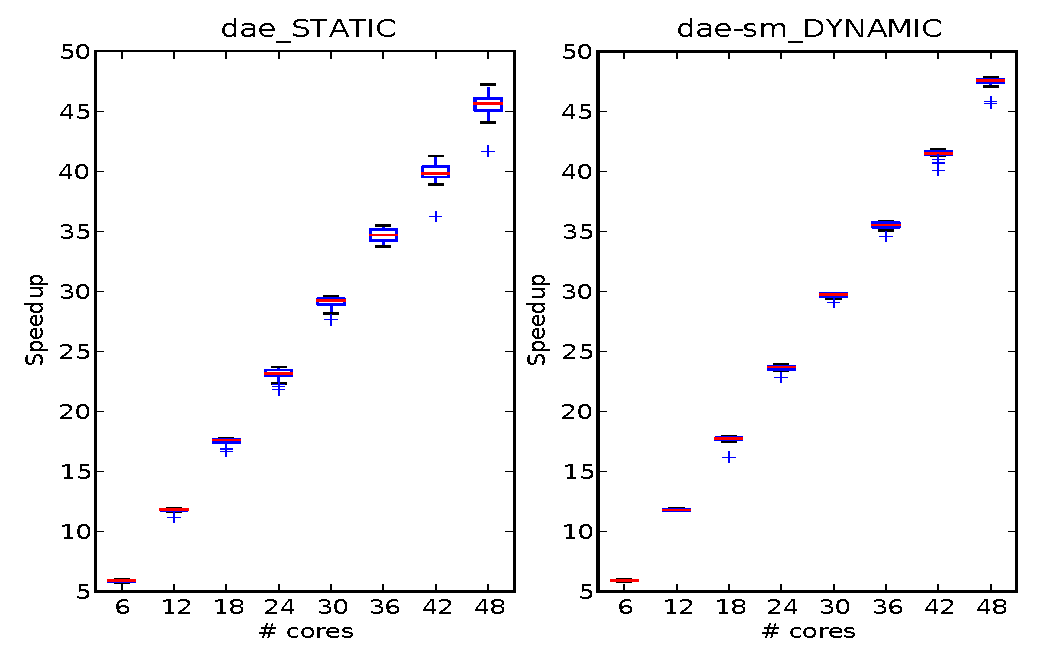
\includegraphics[width=0.45\textwidth]{images/EXP2_Speed_up_IPC6_TEMPO_OPENSTACKS_17_S96_nosm-static_sm_vs_dynamic.pdf}
\caption{Speedup of \DAEYAHSP\ relative to the number of processors, on \OPENSTACKS-17.
On the left: with local memoization and the static parallelization scheme, on the right: with shared memoization and the dynamic parallelization scheme.}
\label{fig:exp2_speedup_core_openstack_17_pop_96_nosm-static_vs_sm-dynamic}
\end{center}
\end{figure}

This observation meets the expected behavior and is classical when considering the parallelization of the evaluation step of an evolutionary algorithm. Nevertheless, the difference among combinations and problems can be seen when considering efficiency.

Figures \ref{fig:exp2_efficiency_core_elevators_12_pop_96} and
\ref{fig:exp2_efficiency_core_openstacks_17_pop_96} shows that for the
benchmark \ELEVATORS-12, shared memoization may perform better for larger
population sizes but that there is no difference between static an dynamic
parallelization schemes. On \OPENSTACKS-17, the dynamic scheme performs
slightly better when used along with the shared memoization.

Since the evaluation times are varying (given the fact that decompositions have
different lengths and that each subproblem may be more or less difficult), by
construction a queue-based scheduling should be more efficient in
average. But the behavior is dependent of the algorithm instance
and ability to avoid premature convergence that would
produce an homogeneous population. Hence the difference between the two
schemes may not be immediately notable.

An explanation for the poor performance gain of using shared memoization might
be that the benefit obtained when memoization is shared among individuals is
lost with the bottleneck due to multiple access locking.

\begin{figure}[H]
\begin{center}
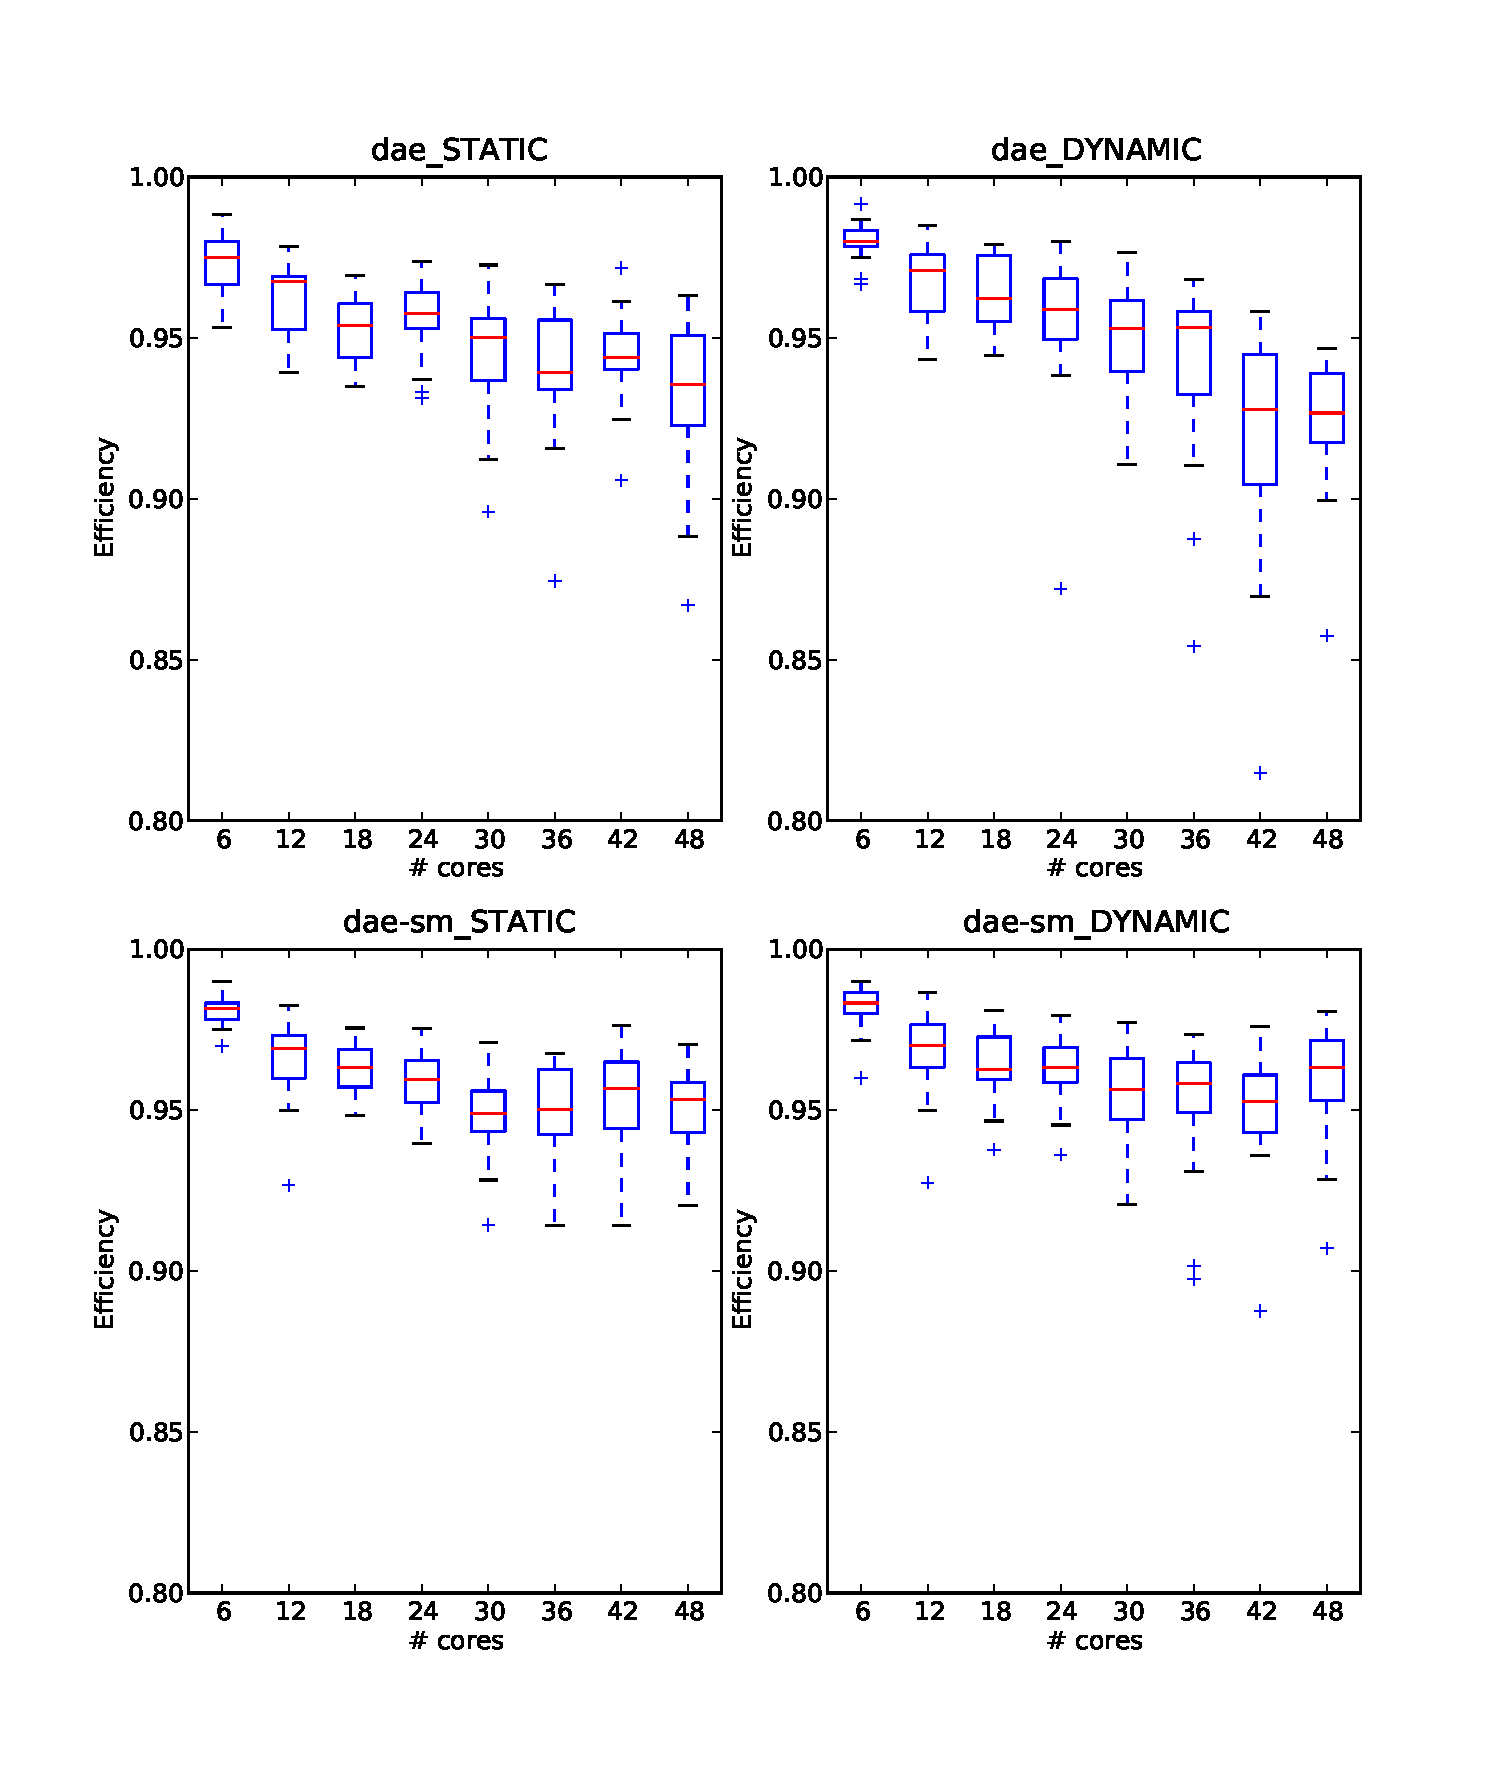
\includegraphics[width=0.47\textwidth]{images/EXP2_Efficiency_IPC6_SEQ_ELEVATORS_12_S96.pdf}
\caption{Efficiency of \DAEYAHSP\ relative to the number of processors, on \ELEVATORS-12.}
\label{fig:exp2_efficiency_core_elevators_12_pop_96}
\end{center}
\end{figure}

\begin{figure}[H]
\begin{center}
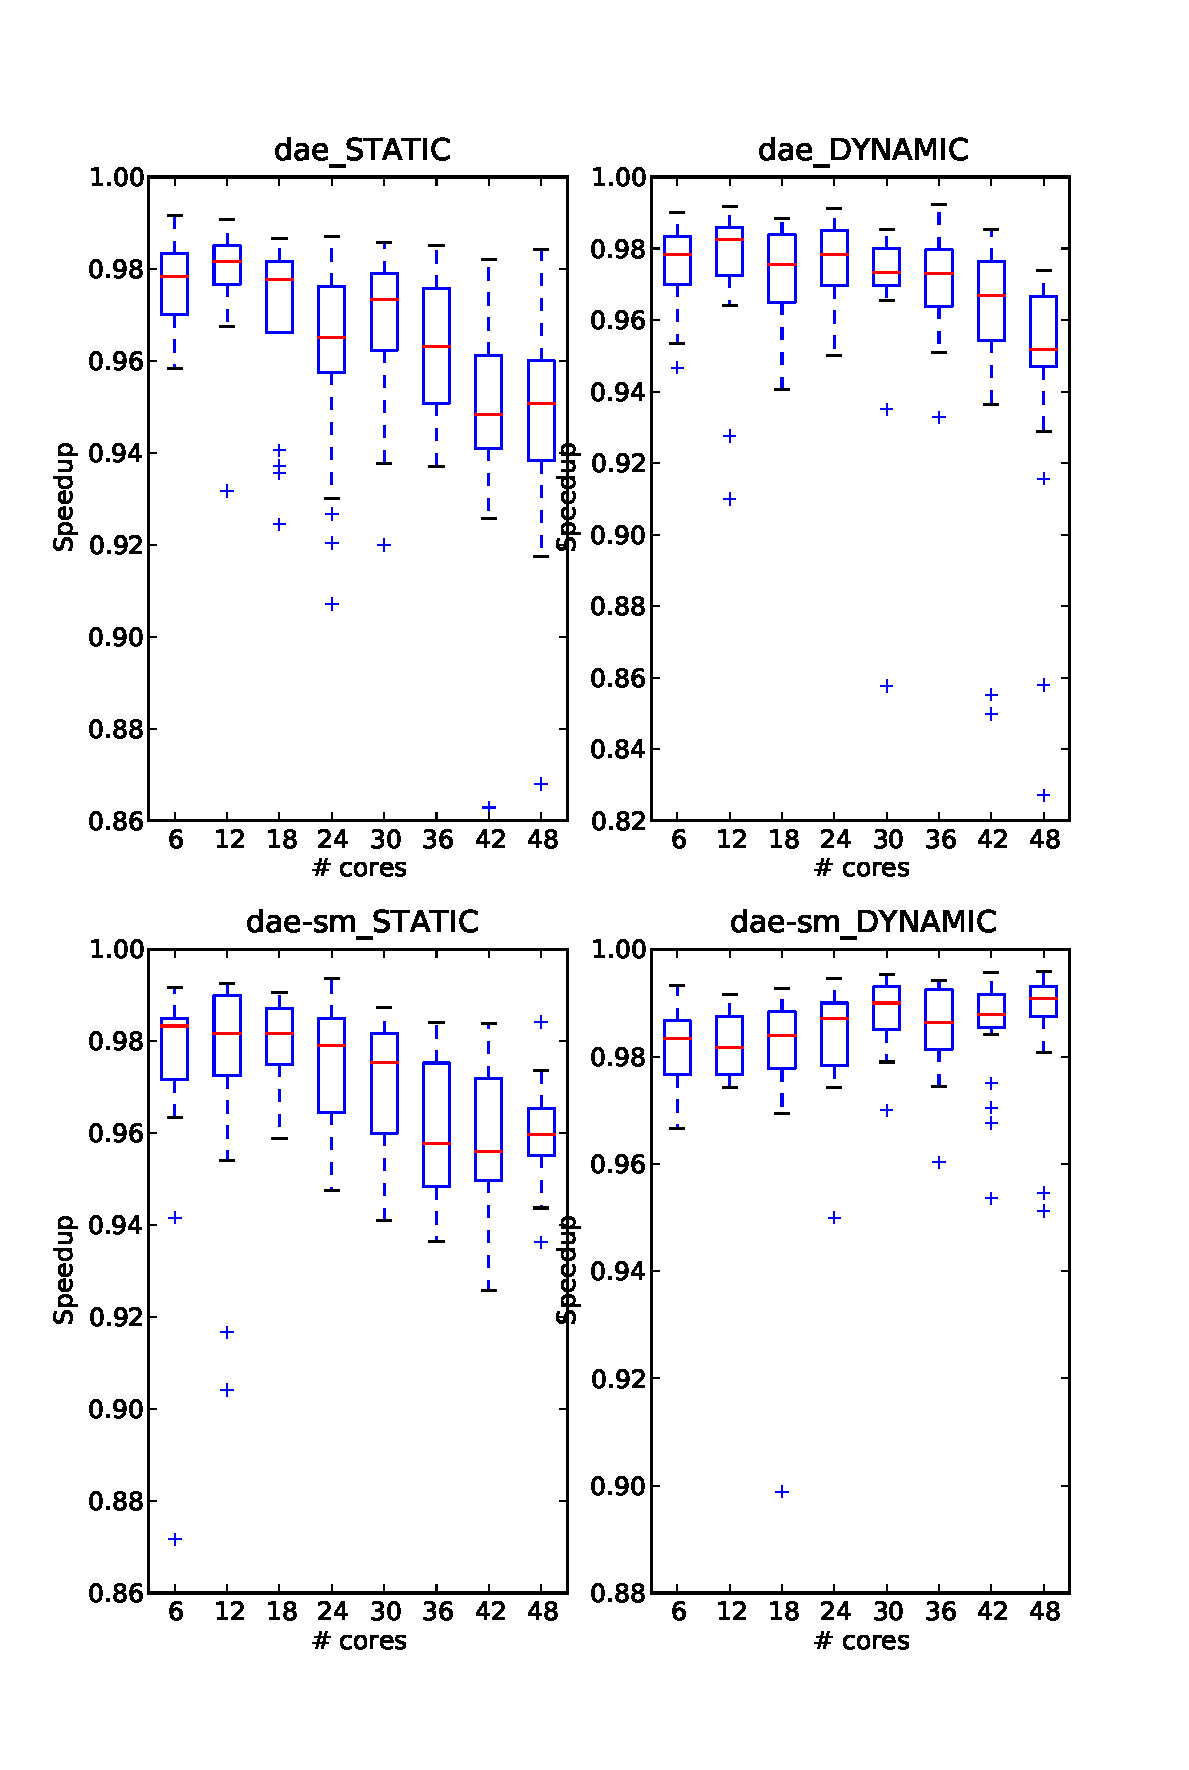
\includegraphics[width=0.47\textwidth]{images/EXP2_Efficiency_IPC6_TEMPO_OPENSTACKS_17_S96.pdf}
\caption{Efficiency of \DAEYAHSP\ relative to the number of processors, on \OPENSTACKS-17.}
\label{fig:exp2_efficiency_core_openstacks_17_pop_96}
\end{center}
\end{figure}

Figures \ref{fig:exp2_totalcost_elevators-12_pop_96} and \ref{fig:exp2_makespan_openstacks-17_pop_96} show that the solution quality remains unaffected by the number of cores used.

\begin{figure}[htpb]
\begin{center}
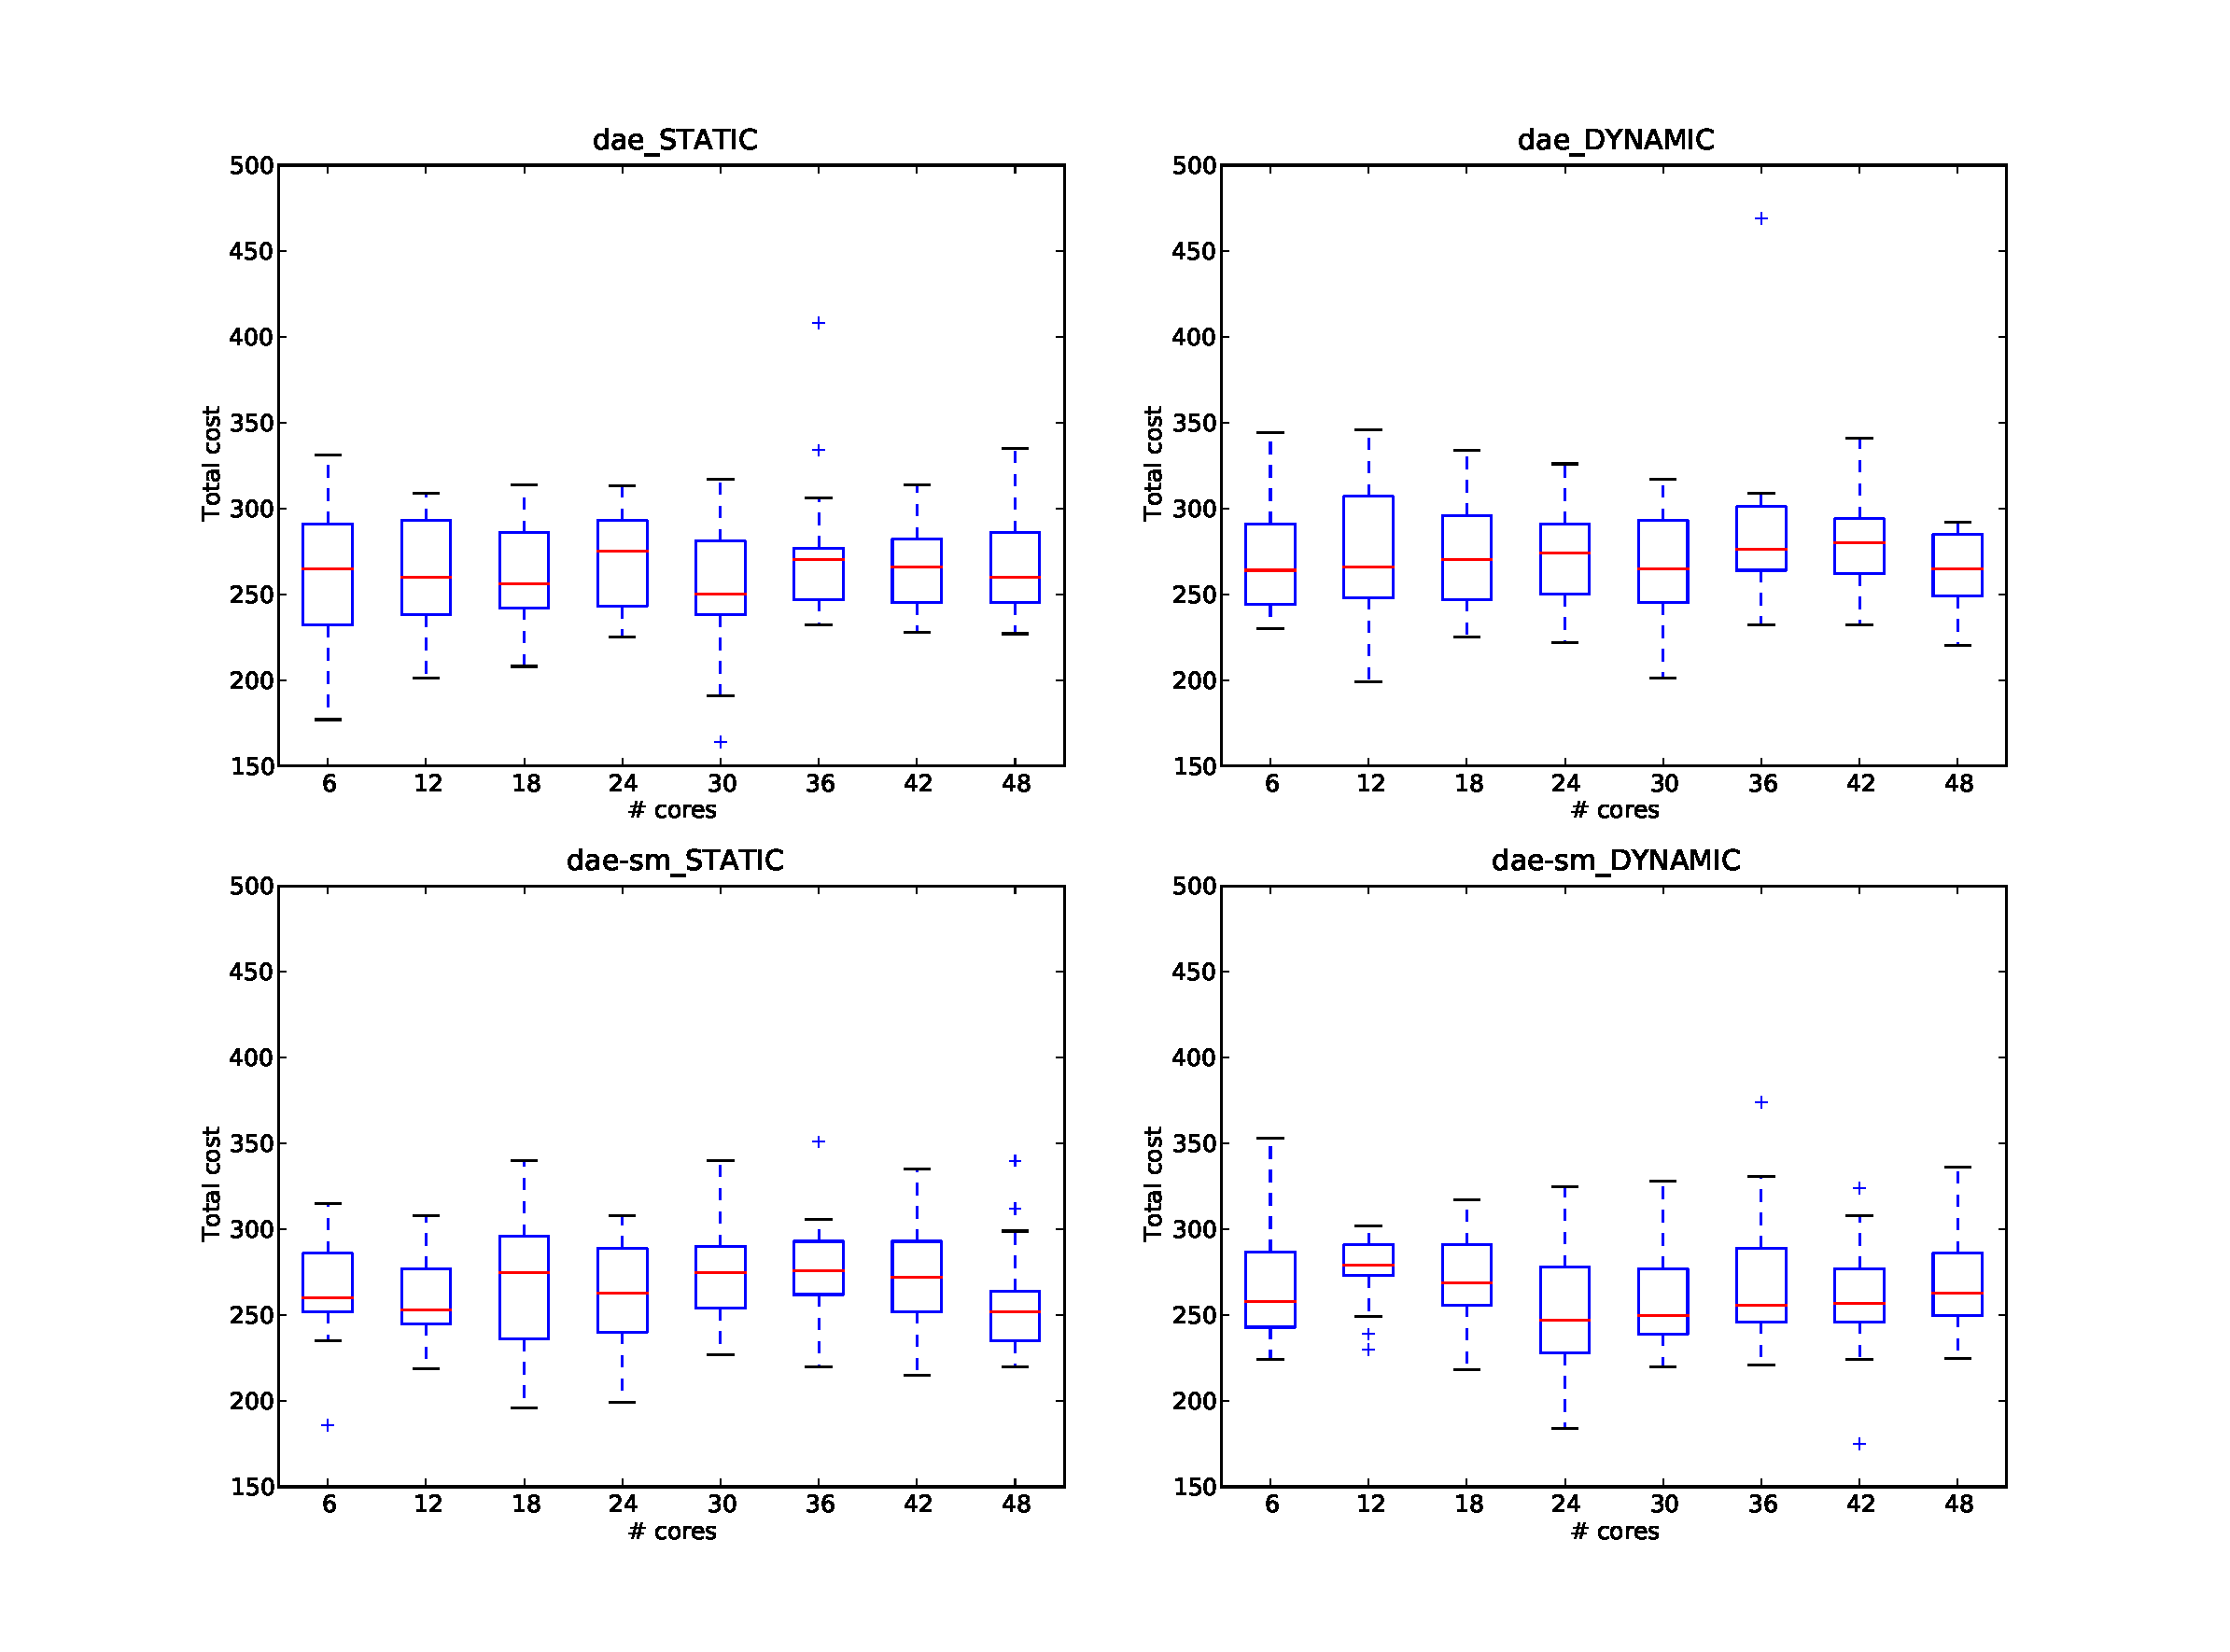
\includegraphics[width=0.5\textwidth]{images/EXP2_Total_cost_IPC6_SEQ_ELEVATORS_12_S96.pdf}
\caption{Total costs of the 4 parallel/memoiza\-tion combinations of \DAEYAHSP\ on \ELEVATORS-12.}
\label{fig:exp2_totalcost_elevators-12_pop_96}
\end{center}
\end{figure}

\begin{figure}[htpb]
\begin{center}
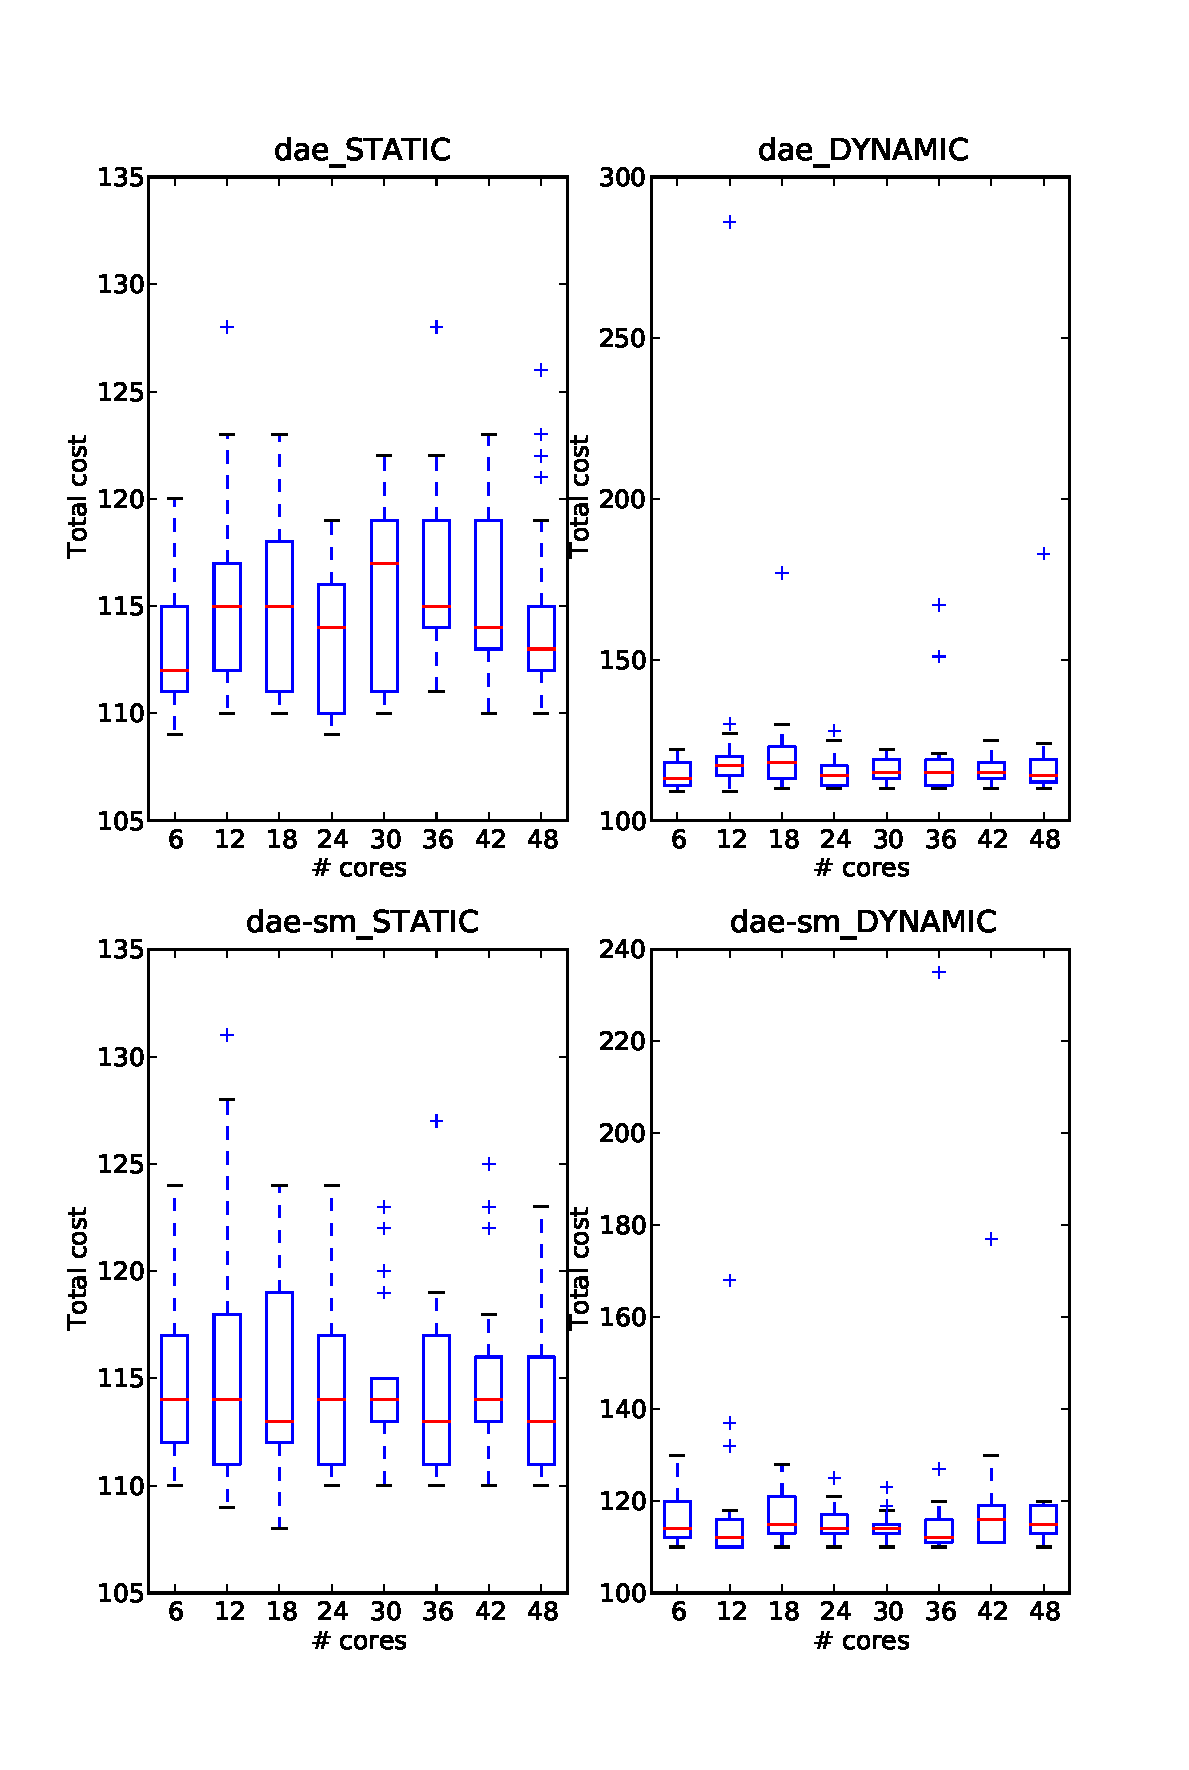
\includegraphics[width=0.5\textwidth]{images/EXP2_Makespan_IPC6_TEMPO_OPENSTACKS_17_S96.pdf}
\caption{Makespans of the 4 parallel/memoiza\-tion combinations of \DAEYAHSP\ on \OPENSTACKS-17.}
\label{fig:exp2_makespan_openstacks-17_pop_96}
\end{center}
\end{figure}

It was expected that the shorter time needed to perform a run would lead
to more restarts within the 30 minutes time contract and thus to an increasing
probability to reach better solutions. Results show that this is not the case.
Again, an explanation for those results is that the
algorithm converge prematurely and cannot find solutions with a sufficiently
high variance to ensure that the probability to find better solutions will
increase with restarts.

\paragraph{Speedup against the population size}
Figure \ref{fig:exp1_efficiency_pop} shows that the efficiency decreases with the size of the population: while being close to the optimum for a size equal to the available number of processors, it rapidly decreases and reaches a plateau for big populations.

\begin{figure}[htpb]
\subfigure[\ELEVATORS-12]{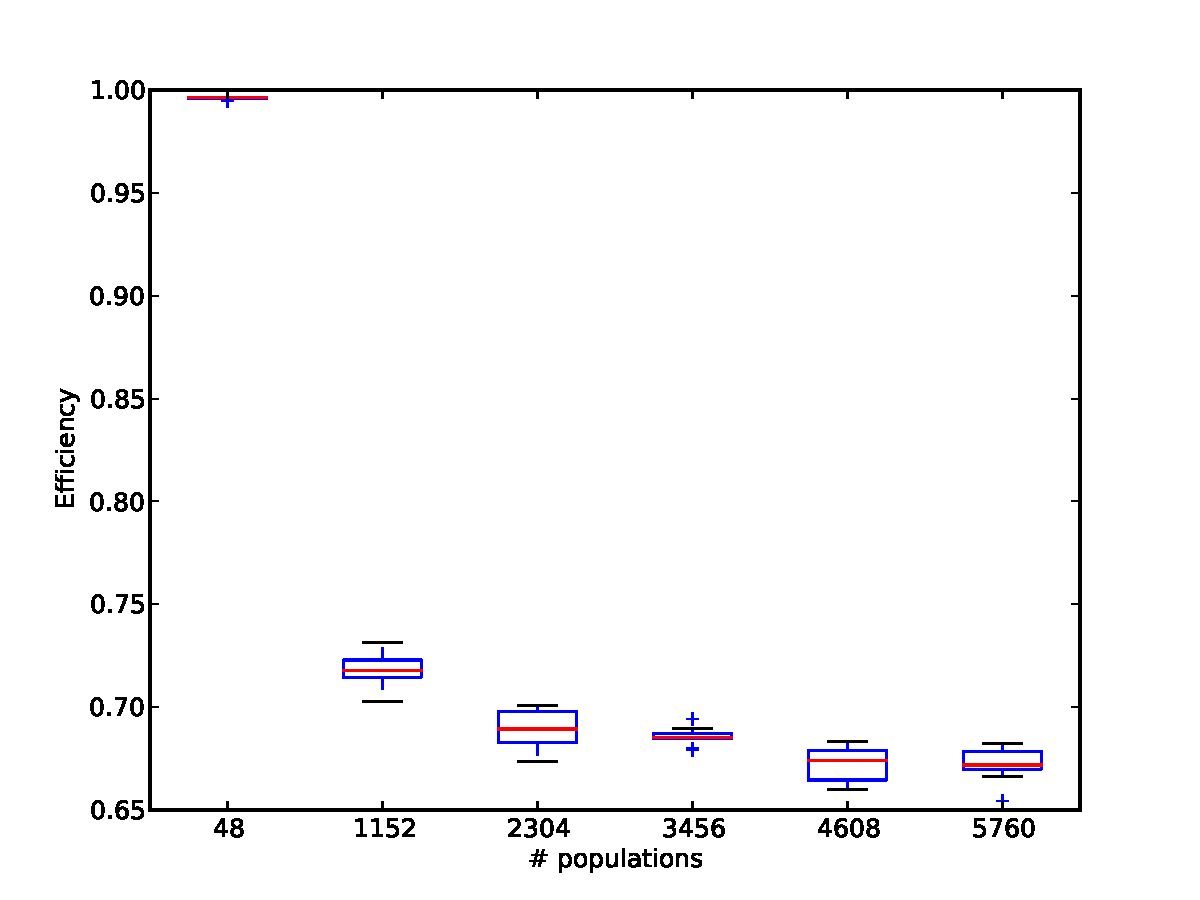
\includegraphics[width=0.23\textwidth]{images/EXP1_Efficiency_IPC6_SEQ_ELEVATORS_12_RESTART_dae-sm_STATIC_.pdf}}
\hfill
\subfigure[\OPENSTACKS-17]{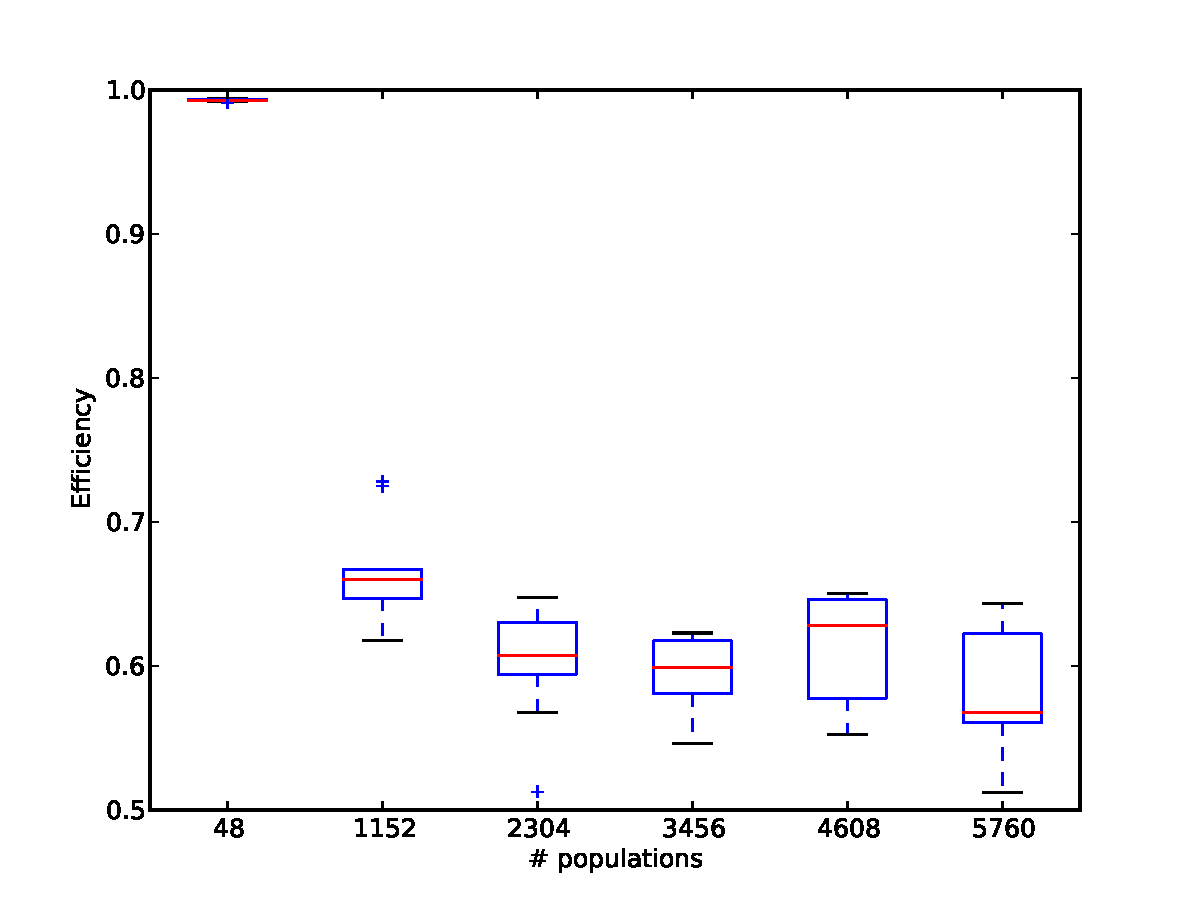
\includegraphics[width=0.23\textwidth]{images/EXP1_Efficiency_IPC6_TEMPO_OPENSTACKS_17_RESTART_dae-sm_STATIC_.pdf}}
\caption{Efficiency of \DAEYAHSP\ relative to the population size.}
\label{fig:exp1_efficiency_pop}
\end{figure}

Using a static parallelization scheme, the decrease in speed\-up is due to the
synchronization step at each generation, when cores have finished the evaluation
of easier decompositions and are waiting for the next generation to occur.

Figure \ref{fig:exp1_totalcost-makespan} shows that no significant difference in
solution qualities can be observed when the population size increases.

\begin{figure}[htpb]
\begin{center}
\subfigure[\ELEVATORS-12]{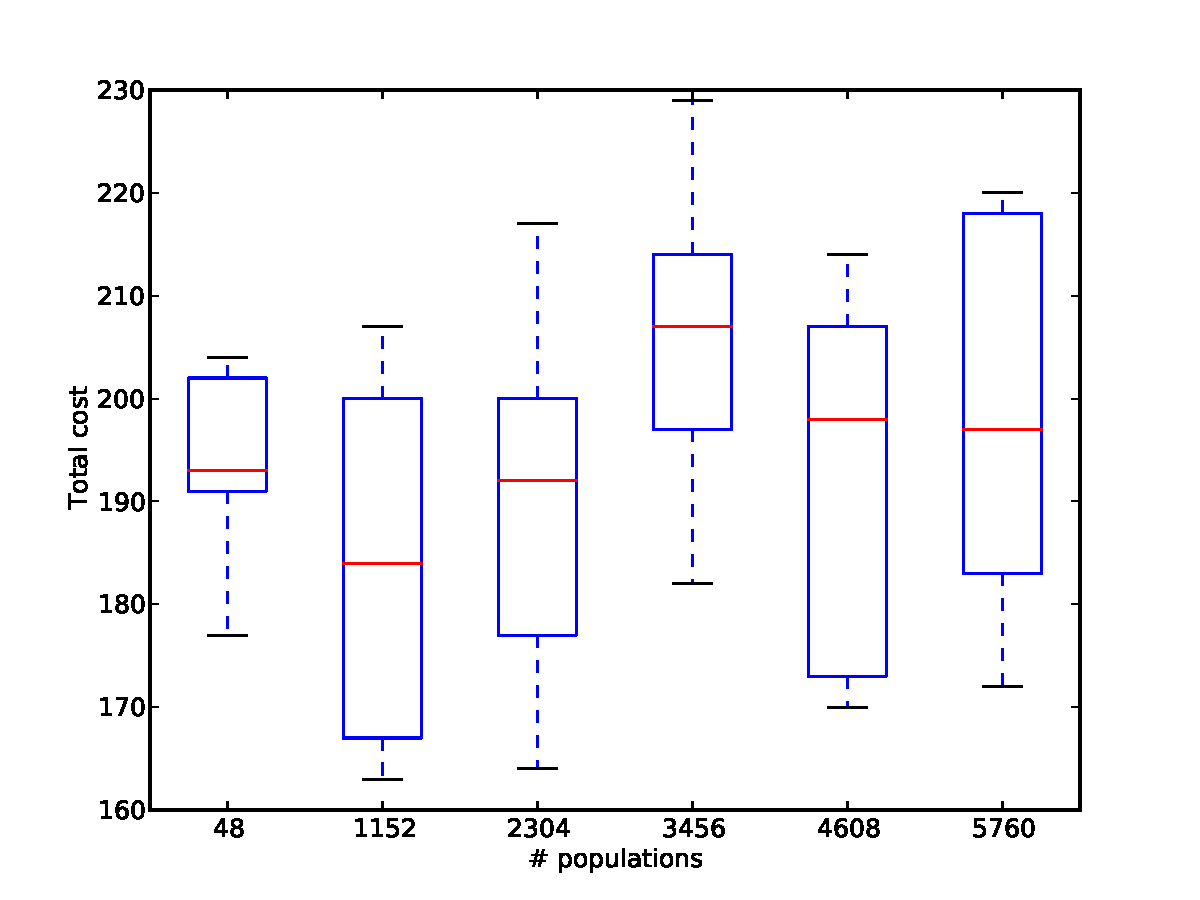
\includegraphics[width=0.23\textwidth]{images/EXP1_Total_cost_IPC6_SEQ_ELEVATORS_12_RESTART_dae-sm_STATIC_.pdf}}
\subfigure[\OPENSTACKS-17]{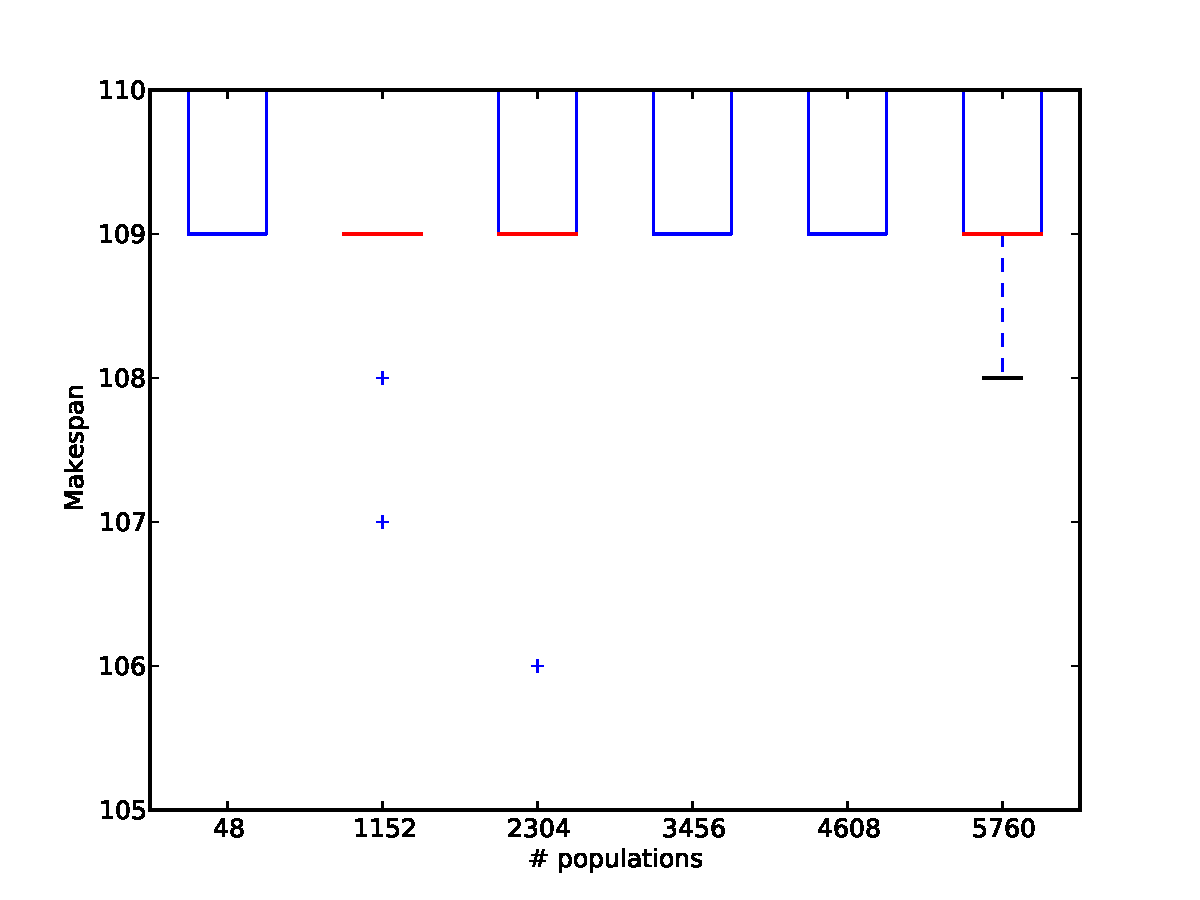
\includegraphics[width=0.23\textwidth]{images/EXP1_Makespan_IPC6_TEMPO_OPENSTACKS_17_RESTART_dae-sm_STATIC_.pdf}}
\end{center}
\caption{Solution plans qualities for increasing population sizes.}
\label{fig:exp1_totalcost-makespan}
\end{figure}

The hypothesis that a larger population would lead to a greater exploration and
thus to a better solution quality is thus not confirmed by experimentation. The
algorithm converges too rapidly, independently of the population size.

\section{Discussion and Conclusion}
We made a proof-of-concept for a shared-memory parallelization of the evaluation
step of the \DAEX\ algorithm, based on the \OPENMP\ directive-based API on a
common 48-core machine. Thanks to the abstraction level provided by the EO
framework, this scheme is immediately available for any evolutionary algorithm
as far as the context of the evaluation functor is thread-local and reentrant.

We obtained on our 48-core Dell Machine, a roughly $\times45$ speedup for the two benchmarks tested, this speedup being the same for all instances.

The dispersion of the measured times is mainly due to the combination of the
steady-state stopping criterion with the stochastic nature of the search, which
may or may not reach a fitness plateau early. The relationship between this
dispersion and the difficulty of the problem solved remains to be explored.

Our results show that the stopping criterion should be chosen carefully, along
with the population size, as it has an impact on the dispersion of the
computation time distribution. Moreover, the population size may indifferently
be chosen small, in order to decrease the computation time.

The dynamic queue mapping management of threads onto cores provides a
significant improvement on a single problem instance, when combined with
shared memoization. Since it has no special impact on the other problem, it
may be preferred, but more tests on other domains are necessary.

The implementation scheme presented here is very simple but works extremely
well. A further development will consist in parallelizing other steps of the
evolutionary loop in particular the offspring generation (which is also
intrinsically parallel) and the selection/replacement operators.

A further research axis deals with the impact on solution quality and in
particular how to take advantage of the parallelization scheme to escape from
premature convergence.

\section{Acknowledgments}
This work is being partially funded by the French National Research Agency through the COSINUS programme, under the research contract DESCARWIN (ANR-09-COSI-002).

\bibliographystyle{abbrv}
\begin{thebibliography}{10}

\bibitem{special:parallelComputing2005}
{Special Issue on OpenMP}.
\newblock {\em Parallel Computing}, 31(10-12):957--1173, 2005.

\bibitem{alba:IEEE2002}
E.~Alba and M.~Tomassini.
\newblock {Parallelism and Evolutionary Algorithms}.
\newblock {\em IEEE Transactions on Evolutionary Computation}, 6(5):443--462,
  2002.

\bibitem{dae:icaps2010}
J.~Biba{\"i}, P.~Sav\'eant, M.~Schoenauer, and V.~Vidal.
\newblock {An Evolutionary Metaheuristic Based on State Decomposition for
  Domain-Independent Satisficing Planning}.
\newblock In {\em $20^{th}$ International Conference on Automated Planning and
  Scheduling (ICAPS-2010)}, pages 18--25. AAAI Press, 2010.

\bibitem{dae:gecco2010}
J.~Biba{\"i}, P.~Sav\'eant, M.~Schoenauer, and V.~Vidal.
\newblock {On the Generality of Parameter Tuning in Evolutionary Planning}.
\newblock In {\em $20^{th}$ Genetic and Evolutionary Computation Conference
  (GECCO'10)}, pages 241--248. ACM Press, 2010.

\bibitem{burns:JAIR2010}
E.~Burns, S.~Lemons, W.~Ruml, and R.~Zhou.
\newblock {Best-First Heuristic Search for Multicore Machines}.
\newblock {\em Journal of Artificial Intelligence Research}, 39:689--743, 2010.

\bibitem{burns:ijcai2009}
E.~Burns, S.~Lemons, R.~Zhou, and W.~Ruml.
\newblock {Best-First Heuristic Search for Multi-Core Machines}.
\newblock In {\em $21^{st}$ International Joint Conference on Artificial
  Intelligence (IJCAI-09)}, pages 449--455. AAAI Press, 2009.

\bibitem{paradiseo:JHeuristics2004}
S.~Cahon, N.~Melab, and E.-G. Talbi.
\newblock {ParadisEO: A Framework for the Reusable Design of Parallel and
  Distributed Metaheuristics}.
\newblock {\em Journal of Heuristics}, 10:357--380, 2004.

\bibitem{PRA-star}
M.~P. Evett, J.~A. Hendler, A.~Mahanti, and D.~S. Nau.
\newblock {{PRA*}: {M}assively Parallel Heuristic Search}.
\newblock {\em Journal of Parallel and Distributed Computing}, 25(2):133--143,
  1995.

\bibitem{pddl:jair2003}
M.~Fox and D.~Long.
\newblock {PDDL2.1: An Extension to PDDL for Expressing Temporal Planning
  Domains}.
\newblock {\em Journal of Artificial Intelligence Research}, 20:61--124, 2003.

\bibitem{gnt04}
M.~Ghallab, D.~Nau, and P.~Traverso.
\newblock {\em {Automated Planning: Theory and Practice}}.
\newblock Morgan Kaufmann, San Francisco, CA, USA, 2004.

\bibitem{h1:aips2000}
P.~Haslum and H.~Geffner.
\newblock Admissible {H}euristics for {O}ptimal {P}lanning.
\newblock In {\em AIPS-2000}, pages 70--82, 2000.

\bibitem{ipc4:jair05}
J.~Hoffmann and S.~Edelkamp.
\newblock {The Deterministic Part of {IPC}-4: {A}n Overview}.
\newblock {\em Journal of Artificial Intelligence Research}, 24:519--579, 2005.

\bibitem{ff:jair01}
J.~Hoffmann and B.~Nebel.
\newblock {The {FF} Planning System: {F}ast Plan Generation Through Heuristic
  Search}.
\newblock {\em Journal of Artificial Intelligence Research}, 14:253--302, 2001.

\bibitem{Huang:openmpGlobalArrays2005}
L.~Huang, B.~Chapman, and Z.~Liu.
\newblock {Towards a More Efficient Implementation of OpenMP for Clusters via
  Translation to Global Arrays}.
\newblock {\em Parallel Computing}, 31:1114--1139, 2005.

\bibitem{HDA-star}
A.~Kishimoto, A.~S. Fukunaga, and A.~Botea.
\newblock {Scalable, Parallel Best-First Search for Optimal Sequential
  Planning}.
\newblock In {\em $19^{th}$ International Conference on Automated Planning and
  Scheduling (ICAPS-2009)}, pages 10--17, 2009.

\bibitem{maitre:gecco2009}
O.~Maitre, L.~Baumes, N.~Lachiche, A.~Corma, and P.~Collet.
\newblock {Coarse Grain Parallelization of Evolutionary Algorithms on GPGPU
  Cards with EASEA}.
\newblock In {\em $19^{th}$ Genetic and Evolutionary Computation Conference
  (GECCO'09)}, pages 1403--1410. ACM Press, 2009.

\bibitem{PFADDD}
R.~Niewiadomski, J.~N. Amaral, and R.~C. Holte.
\newblock {Sequential and Parallel Algorithms for Frontier {A}* with Delayed
  Duplicate Detection}.
\newblock In {\em $21^{st}$ National Conference on Artificial Intelligence
  (AAAI-2006)}, 2006.

\bibitem{lama:jair2010}
S.~Richter and M.~Westphal.
\newblock {The {LAMA} Planner: {G}uiding Cost-Based Anytime Planning with
  Landmarks}.
\newblock {\em Journal of Artificial Intelligence Research}, 39:127--177, 2010.

\bibitem{rintanen:acai2010}
J.~Rintanen.
\newblock {Heuristic Planning with SAT: Beyond Uninformed Depth-First Search}.
\newblock In {\em $23^{rd}$ Australasian Conference on Artificial Intelligence
  (ACAI-2010)}, pages 415--424, 2010.

\bibitem{TDS}
J.~W. Romein, A.~Plaat, H.~E. Bal, and J.~Schaeffer.
\newblock {Transposition Table Driven Work Scheduling in Distributed Search}.
\newblock In {\em $16^{th}$ National Conference on Artificial Intelligence
  (AAAI-1999)}, pages 725--731, 1999.

\bibitem{dae:evocop2006}
M.~Schoenauer, P.~Sav\'eant, and V.~Vidal.
\newblock {Divide-and-Evolve: a New Memetic Scheme for Domain-Independent
  Temporal Planning}.
\newblock In J.~Gottlieb and G.~Raidl, editors, {\em $6^{th}$ European
  Conference on Evolutionary Computation in Combinatorial Optimization
  (EvoCOP'06)}, pages 247--260. Springer Verlag, 2006.

\bibitem{dovetailing}
R.~Valenzano, N.~Sturtevant, J.~Schaeffer, K.~Buro, and A.~Kishimoto.
\newblock {Simultaneously Searching with Multiple Settings: {A}n Alternative to
  Parameter Tuning for Suboptimal Single-Agent Search Algorithms}.
\newblock In {\em $20^{th}$ International Conference on Automated Planning and
  Scheduling (ICAPS-2010)}, pages 177--184, 2010.

\bibitem{yahsp:icaps2004}
V.~Vidal.
\newblock {A Lookahead Strategy for Heuristic Search Planning}.
\newblock In {\em $14^{th}$ International Conference on Automated Planning and
  Scheduling (ICAPS-2004)}, pages 150--159. AAAI Press, 2004.

\bibitem{vidal:socs2010}
V.~Vidal, L.~Bordeaux, and Y.~Hamadi.
\newblock {Adaptive K-Parallel Best-First Search: A simple but Efficient
  Algorithm for Multi-Core Domain-Independent Planning}.
\newblock In {\em $3^{rd}$ Annual Symposium on Combinatorial Search (SOCS'10)},
  pages 100--107. AAAI Press, 2010.

\end{thebibliography}

\end{document}
